% ============================================================================
% IEEE Standard Report – Patient Management System
% Course: CO2060 | University of Peradeniya
% ============================================================================
\documentclass[conference]{IEEEtran}

% ─── Packages ───────────────────────────────────────────────────────────────
\usepackage{cite}
\usepackage{amsmath,amssymb,amsfonts}
\usepackage{algorithmic}
\usepackage{graphicx}
\usepackage{textcomp}
\usepackage{xcolor}
\usepackage{hyperref}
\usepackage{listings}
\usepackage{tabularx}
\usepackage{booktabs}
\usepackage{float}
\usepackage{enumitem}
\usepackage{url}

% ─── Listings style for code snippets ───────────────────────────────────────
\lstset{
  basicstyle=\ttfamily\footnotesize,
  breaklines=true,
  frame=single,
  captionpos=b,
  numbers=left,
  numberstyle=\tiny\color{gray},
  keywordstyle=\color{blue},
  commentstyle=\color{green!50!black},
  stringstyle=\color{red!60!black},
}

% ─── Hyperlink styling ─────────────────────────────────────────────────────
\hypersetup{
  colorlinks=true,
  linkcolor=blue,
  citecolor=blue,
  urlcolor=blue
}

\def\BibTeX{{\rm B\kern-.05em{\sc i\kern-.025em b}\kern-.08em
    T\kern-.1667em\lower.7ex\hbox{E}\kern-.125emX}}

% ============================================================================
\begin{document}

% ─── Title ──────────────────────────────────────────────────────────────────
\title{Patient Management System: A Web-Based Solution for Centralized Healthcare Data Management}

% ─── Authors ────────────────────────────────────────────────────────────────
\author{
  \IEEEauthorblockN{S.M.L.E.~Senadhipathi}
  \IEEEauthorblockA{
    \textit{Department of Computer Engineering} \\
    \textit{University of Peradeniya} \\
    Peradeniya, Sri Lanka \\
    e22364@eng.pdn.ac.lk}
  \and
  \IEEEauthorblockN{D.D.S.K.~Gunawardhana}
  \IEEEauthorblockA{
    \textit{Department of Computer Engineering} \\
    \textit{University of Peradeniya} \\
    Peradeniya, Sri Lanka \\
    e22125@eng.pdn.ac.lk}
  \and
  \IEEEauthorblockN{G.K.M.~Jayanga}
  \IEEEauthorblockA{
    \textit{Department of Computer Engineering} \\
    \textit{University of Peradeniya} \\
    Peradeniya, Sri Lanka \\
    e22159@eng.pdn.ac.lk}
  \and
  \IEEEauthorblockN{D.D.~Abeysinghe}
  \IEEEauthorblockA{
    \textit{Department of Computer Engineering} \\
    \textit{University of Peradeniya} \\
    Peradeniya, Sri Lanka \\
    e22004@eng.pdn.ac.lk}
}

\maketitle

% ============================================================================
% ABSTRACT
% ============================================================================
\begin{abstract}
Healthcare facilities worldwide continue to face significant challenges arising from paper-based record-keeping, fragmented patient information, appointment scheduling conflicts, and limited accessibility to medical histories. These persistent issues lead to treatment delays, data loss, and a deteriorated patient experience. This paper presents the design and implementation of a \textbf{Patient Management System (PMS)}---a comprehensive, web-based application engineered to centralize and streamline the management of patient records, medical histories, appointments, billing, pharmacy operations, and clinical workflows. The system employs a modern three-tier architecture utilizing \textbf{React} for the frontend, \textbf{Spring Boot (Java)} for the backend, and \textbf{PostgreSQL} as the relational database. Security is enforced through \textbf{JSON Web Token (JWT)} authentication, \textbf{BCrypt} password hashing, role-based access control (RBAC) spanning ten distinct user roles, and comprehensive audit logging. Real-time notifications are delivered via \textbf{WebSocket} integration. The system has been deployed with the frontend hosted on \textbf{Vercel} and the backend on \textbf{Render}, demonstrating a scalable, cloud-native deployment strategy. Evaluation results indicate that the PMS significantly improves data accuracy, reduces manual workload, and supports enhanced clinical decision-making.
\end{abstract}

% ─── Keywords ───────────────────────────────────────────────────────────────
\begin{IEEEkeywords}
Patient Management System, Electronic Health Records, Spring Boot, React, JWT Authentication, Role-Based Access Control, WebSocket, Healthcare Information System, RESTful API
\end{IEEEkeywords}

% ============================================================================
% I. INTRODUCTION
% ============================================================================
\section{Introduction}

The global healthcare industry is undergoing a rapid digital transformation, driven by the need to improve patient outcomes, reduce operational costs, and enhance the accessibility of medical services~\cite{b1}. Despite these advances, many healthcare facilities---particularly in developing regions---continue to rely on paper-based record systems that are prone to data loss, duplication, and unauthorized access~\cite{b2}.

Traditional patient management approaches suffer from several critical limitations:
\begin{itemize}[leftmargin=*]
  \item \textbf{Data Fragmentation:} Patient information is scattered across multiple departments, making it difficult to obtain a holistic view of a patient's medical history.
  \item \textbf{Appointment Conflicts:} Manual scheduling processes lead to double bookings, missed appointments, and inefficient utilization of healthcare provider time.
  \item \textbf{Limited Accessibility:} Paper records cannot be accessed remotely, hindering telemedicine and inter-departmental collaboration.
  \item \textbf{Security Vulnerabilities:} Physical records are susceptible to unauthorized access, loss, and damage.
  \item \textbf{Lack of Audit Trails:} Manual systems offer no mechanism for tracking who accessed or modified patient data.
\end{itemize}

The \textbf{Patient Management System (PMS)} presented in this paper addresses these challenges by providing a centralized, secure, and user-friendly web-based platform. The system supports ten distinct user roles---Super Admin, Admin, Management, Doctor, Nurse, Receptionist, Pharmacist, Lab Technician, Billing Staff, and Patient---each with tailored dashboards and access permissions.

The primary contributions of this work are:
\begin{enumerate}[leftmargin=*]
  \item A comprehensive, role-based healthcare management platform with ten specialized user interfaces.
  \item A secure authentication and authorization framework using JWT tokens with refresh token rotation and BCrypt password hashing.
  \item Real-time notification delivery through WebSocket integration.
  \item A scalable, cloud-native deployment architecture using Vercel and Render.
  \item Database version control through Flyway migrations ensuring schema consistency across environments.
\end{enumerate}

The remainder of this paper is organized as follows: Section~II reviews related work. Section~III describes the system architecture. Section~IV presents the detailed software design. Section~V discusses the implementation. Section~VI covers testing and evaluation. Section~VII presents results and discussion. Section~VIII concludes the paper and outlines future work.

% ============================================================================
% II. LITERATURE REVIEW
% ============================================================================
\section{Literature Review}

\subsection{Electronic Health Record (EHR) Systems}
Electronic Health Record systems have been extensively studied as a means to improve healthcare delivery. Adler-Milstein et al.~\cite{b1} demonstrated that EHR adoption significantly reduces medical errors and improves care coordination. However, many commercial EHR solutions such as Epic and Cerner are prohibitively expensive for smaller healthcare facilities~\cite{b3}.

\subsection{Open-Source Healthcare Solutions}
Open-source alternatives like OpenMRS~\cite{b4} and GNU Health~\cite{b5} have gained traction in resource-constrained settings. While these systems provide core functionality, they often lack modern user interfaces, real-time communication capabilities, and comprehensive role-based access control mechanisms suitable for diverse healthcare environments.

\subsection{Web-Based Healthcare Applications}
Recent studies have explored the use of modern web technologies for healthcare applications. Kumar et al.~\cite{b6} proposed a React-based patient portal that demonstrated improved patient engagement. Similarly, Spring Boot has been widely adopted for building secure, scalable backend services in healthcare~\cite{b7}.

\subsection{Security in Healthcare Information Systems}
Healthcare data security is governed by stringent regulations such as HIPAA~\cite{b8}. JWT-based authentication has emerged as a preferred approach for stateless, scalable authentication in web applications~\cite{b9}. Role-based access control (RBAC) provides granular permission management, which is essential in multi-stakeholder healthcare environments~\cite{b10}.

\subsection{Gap Analysis}
Existing solutions often focus on a subset of healthcare workflows---patient records, appointments, or billing---without providing an integrated platform that addresses the complete operational needs of a healthcare facility. Furthermore, many systems lack real-time notification capabilities and comprehensive audit logging. The PMS presented in this paper bridges these gaps by offering a unified platform with broad functional coverage, real-time communication, and robust security features.

% ============================================================================
% III. SYSTEM ARCHITECTURE
% ============================================================================
\section{System Architecture}

The PMS follows a \textbf{three-tier client-server architecture}, separating presentation, business logic, and data persistence concerns. Fig.~\ref{fig:architecture} illustrates the high-level system architecture.

\subsection{Presentation Tier (Frontend)}
The frontend is built using \textbf{React} with \textbf{React Router} for client-side navigation. It provides role-specific dashboards for each of the ten user roles. Key frontend features include:
\begin{itemize}[leftmargin=*]
  \item Responsive design for desktop and mobile devices
  \item Role-based dashboard rendering
  \item Real-time notification display via WebSocket
  \item Form validation and error handling
  \item State management using React Context API
\end{itemize}

\subsection{Business Logic Tier (Backend)}
The backend is developed using \textbf{Spring Boot 3.x} with Java, following a modular, package-by-feature architecture. Each feature module (e.g., \texttt{patient}, \texttt{appointment}, \texttt{billing}) contains its own controller, service, repository, DTO, and entity layers. The backend modules include:
\begin{itemize}[leftmargin=*]
  \item \texttt{auth} -- Authentication and JWT token management
  \item \texttt{patient} -- Patient CRUD operations and vitals tracking
  \item \texttt{doctor} -- Doctor profile management
  \item \texttt{nurse} -- Nurse workflow and vitals recording
  \item \texttt{appointment} -- Appointment scheduling and management
  \item \texttt{medicalrecord} -- Medical records and clinical notes
  \item \texttt{billing} -- Invoice generation and payment tracking
  \item \texttt{pharmacy} -- Prescription and medication management
  \item \texttt{notification} -- Real-time notification service
  \item \texttt{audit} -- Audit logging for compliance
  \item \texttt{admin} -- Administrative operations
  \item \texttt{management} -- Staff and user management
  \item \texttt{profilechange} -- Profile change request workflows
  \item \texttt{file} -- File upload and download services
  \item \texttt{config} -- Security, CORS, WebSocket, and rate limiting configurations
\end{itemize}

\subsection{Data Tier (Database)}
The system uses \textbf{PostgreSQL} as the primary relational database. Schema migrations are managed through \textbf{Flyway}, ensuring version-controlled, repeatable database deployments. The migration history spans 16 versions (V1 through V16), covering the initial schema, refresh tokens, billing, audit logs, notifications, nurse workflows, pharmacy/medicines, and various schema refinements.

\subsection{Communication Protocols}
\begin{itemize}[leftmargin=*]
  \item \textbf{REST API:} All client-server communication uses RESTful HTTP endpoints with JSON payloads.
  \item \textbf{WebSocket:} Real-time notifications are delivered through STOMP over WebSocket, configured via \texttt{WebSocketConfig}.
  \item \textbf{HTTPS:} All production traffic is encrypted using TLS with HSTS enforcement.
\end{itemize}

\begin{figure}[H]
  \centering
  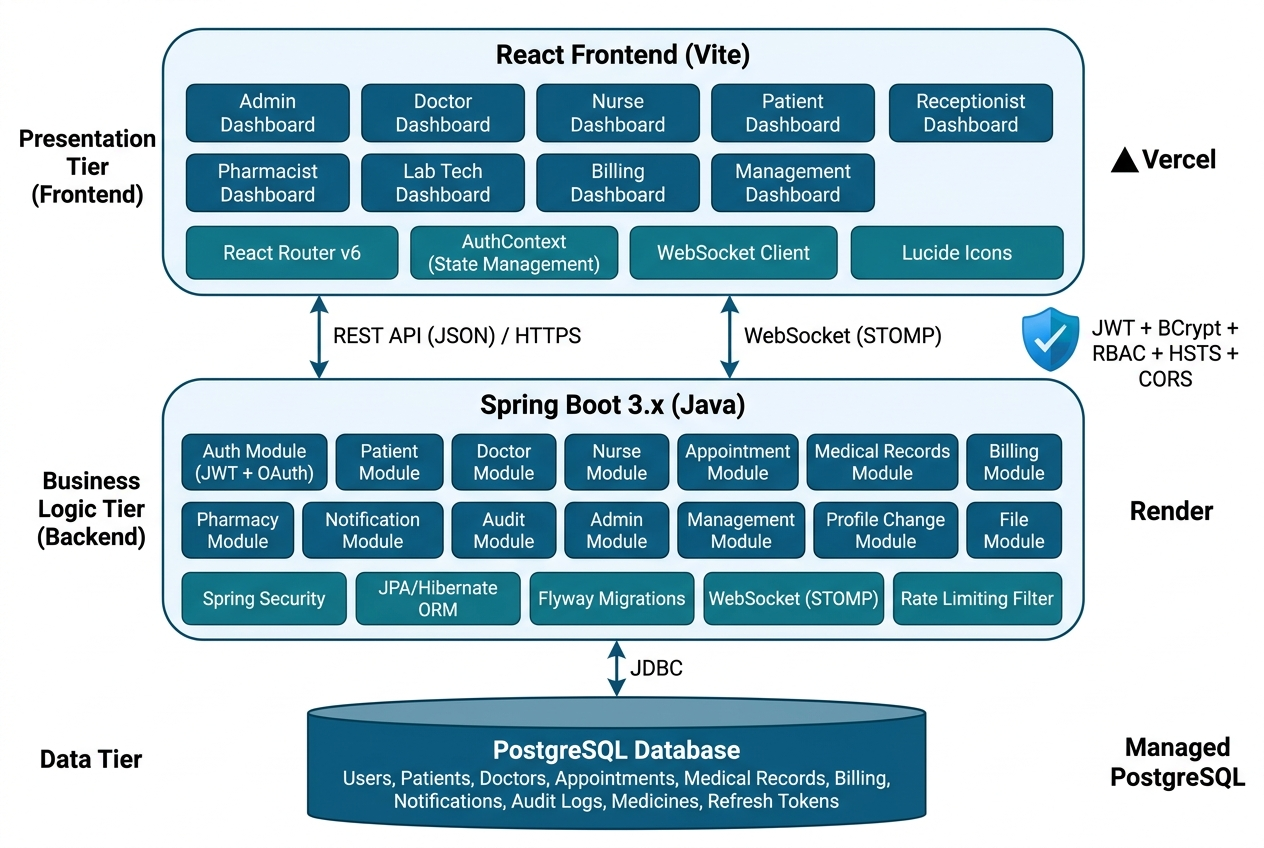
\includegraphics[width=\columnwidth]{images/architecture_diagram.jpg}
  \caption{High-level system architecture of the Patient Management System.}
  \label{fig:architecture}
\end{figure}

% ============================================================================
% IV. SOFTWARE DESIGN
% ============================================================================
\section{Software Design}

\subsection{Module Design}

The system is organized into six primary functional modules, each addressing a specific domain within healthcare operations.

\subsubsection{Patient Management Module}
This module handles the complete lifecycle of patient data, including:
\begin{itemize}[leftmargin=*]
  \item Patient registration with demographic and emergency contact information
  \item Vital signs tracking (blood pressure, heart rate, temperature, oxygen saturation, respiratory rate, height, weight)
  \item Admission and discharge management with status tracking
  \item Medical history, allergy, and current medication records
  \item Critical patient status flagging
  \item Duplicate patient detection
\end{itemize}

\subsubsection{Medical Records Module}
Clinical documentation is managed through structured medical records containing:
\begin{itemize}[leftmargin=*]
  \item Diagnosis and treatment documentation
  \item Prescription management
  \item Test results and lab reports
  \item File attachments for medical documents
  \item Record type categorization
\end{itemize}

\subsubsection{Appointment Management Module}
The appointment system provides:
\begin{itemize}[leftmargin=*]
  \item Scheduling with date, time, and duration specification
  \item Status management (Scheduled, Completed, Cancelled, No-Show)
  \item Doctor availability tracking
  \item Reason for visit documentation
  \item Appointment history and attendance records
\end{itemize}

\subsubsection{User and Access Control Module}
Access control is implemented through a comprehensive RBAC system with ten roles as shown in Table~\ref{tab:roles}.

\begin{table}[H]
\centering
\caption{System Roles and Access Levels}
\label{tab:roles}
\begin{tabularx}{\columnwidth}{lX}
\toprule
\textbf{Role} & \textbf{Access Level} \\
\midrule
Super Admin    & Full unrestricted access to all system features \\
Admin          & User management, reports, audit logs \\
Management     & Staff management (excluding admin accounts) \\
Doctor         & Full clinical access, patient records, prescriptions \\
Nurse          & Record vitals, assist doctors, clinical workflows \\
Receptionist   & Book appointments, register patients \\
Pharmacist     & Manage prescriptions and medications \\
Lab Technician & Enter and manage lab results \\
Billing Staff  & Billing, invoicing, and payment processing \\
Patient        & View own records, appointments, and notifications \\
\bottomrule
\end{tabularx}
\end{table}

\subsubsection{Billing and Insurance Module}
The billing module supports:
\begin{itemize}[leftmargin=*]
  \item Invoice generation linked to appointments and services
  \item Payment tracking and billing history
  \item Insurance information management
  \item Integration with pharmacy for medication billing
\end{itemize}

\subsubsection{Notification Module}
Real-time notifications are categorized into seven types:
\begin{itemize}[leftmargin=*]
  \item \texttt{APPOINTMENT} -- Appointment reminders and updates
  \item \texttt{LAB\_RESULT} -- Lab result availability alerts
  \item \texttt{CRITICAL\_ALERT} -- Critical patient status notifications
  \item \texttt{PRESCRIPTION} -- Prescription-related notifications
  \item \texttt{MEDICATION} -- Medication reminders
  \item \texttt{SYSTEM\_ALERT} -- System-wide announcements
  \item \texttt{MESSAGE} -- General inter-user messages
\end{itemize}

\subsection{Database Design}

The relational database schema comprises the following key entities and their relationships:

\subsubsection{Core Entities}
\begin{itemize}[leftmargin=*]
  \item \textbf{Users:} Stores user credentials, contact information, role assignment, and active status.
  \item \textbf{Patients:} Extended user profile with clinical data including vitals, admission details, and medical history.
  \item \textbf{Doctors:} Specialized profile with specialization, license number, department, consultation fee, and availability.
  \item \textbf{Appointments:} Links patients and doctors with scheduling and status information.
  \item \textbf{Medical Records:} Clinical documentation linked to patients and doctors.
  \item \textbf{Billing:} Financial records for services rendered.
  \item \textbf{Notifications:} Typed notification records for real-time delivery.
  \item \textbf{Audit Logs:} Comprehensive activity tracking for compliance.
  \item \textbf{Refresh Tokens:} Secure token storage for JWT refresh rotation.
  \item \textbf{Profile Change Requests:} Workflow for managing user profile modifications.
  \item \textbf{Medicines:} Pharmacy inventory with pricing information.
\end{itemize}

\subsubsection{Entity Relationships}
Key relationships in the database include:
\begin{itemize}[leftmargin=*]
  \item One User $\rightarrow$ One Patient (1:1)
  \item One User $\rightarrow$ One Doctor (1:1)
  \item One Patient $\rightarrow$ Many Appointments (1:N)
  \item One Doctor $\rightarrow$ Many Appointments (1:N)
  \item One Patient $\rightarrow$ Many Medical Records (1:N)
  \item One Doctor $\rightarrow$ Many Medical Records (1:N)
\end{itemize}

Performance optimization is achieved through database indexes on frequently queried columns, including \texttt{patients.user\_id}, \texttt{appointments.patient\_id}, \texttt{appointments.doctor\_id}, \texttt{medical\_records.patient\_id}, and \texttt{medical\_records.doctor\_id}.

\subsection{Security Design}

The security architecture implements defense-in-depth principles:

\subsubsection{Authentication}
\begin{itemize}[leftmargin=*]
  \item \textbf{JWT Authentication:} Stateless token-based authentication with configurable expiration.
  \item \textbf{Refresh Token Rotation:} Secure refresh token mechanism to maintain sessions without re-authentication.
  \item \textbf{Password Hashing:} BCrypt with a strength factor of 12 for password storage.
  \item \textbf{Google OAuth Integration:} Support for third-party authentication via Google.
\end{itemize}

\subsubsection{Authorization}
\begin{itemize}[leftmargin=*]
  \item \textbf{Method-Level Security:} Spring Security's \texttt{@PreAuthorize} annotations enforce role-based access at the controller level.
  \item \textbf{URL-Based Security:} Endpoint-level access control configured in \texttt{SecurityConfig}.
  \item \textbf{Stateless Sessions:} Session management configured as \texttt{STATELESS} to prevent session fixation attacks.
\end{itemize}

\subsubsection{Transport Security}
\begin{itemize}[leftmargin=*]
  \item \textbf{HTTPS Enforcement:} HTTP Strict Transport Security (HSTS) with a 1-year max-age and subdomain inclusion.
  \item \textbf{CORS Configuration:} Strict cross-origin resource sharing with whitelisted origins.
  \item \textbf{Security Headers:} X-Frame-Options (DENY), X-Content-Type-Options (nosniff), and strict referrer policy.
\end{itemize}

\subsubsection{Additional Security Measures}
\begin{itemize}[leftmargin=*]
  \item \textbf{Rate Limiting:} \texttt{RateLimitingFilter} prevents brute-force attacks and API abuse.
  \item \textbf{Audit Logging:} Asynchronous audit log recording for all sensitive operations.
  \item \textbf{Input Validation:} DTO-level validation to prevent injection attacks.
\end{itemize}

% ============================================================================
% V. IMPLEMENTATION
% ============================================================================
\section{Implementation}

\subsection{Development Environment and Tools}
Table~\ref{tab:techstack} summarizes the technology stack employed in the development of the PMS.

\begin{table}[H]
\centering
\caption{Technology Stack}
\label{tab:techstack}
\begin{tabularx}{\columnwidth}{lX}
\toprule
\textbf{Component} & \textbf{Technology} \\
\midrule
Frontend Framework   & React 18.x with JSX \\
Frontend Routing     & React Router v6 \\
Frontend Icons       & Lucide React \\
Backend Framework    & Spring Boot 3.x (Java) \\
ORM                  & Spring Data JPA / Hibernate \\
Database             & PostgreSQL \\
DB Migrations        & Flyway \\
Authentication       & Spring Security + JWT \\
Password Hashing     & BCrypt (strength 12) \\
Real-Time Comm.      & WebSocket (STOMP protocol) \\
Build Tool           & Maven (backend), Vite (frontend) \\
Version Control      & Git / GitHub \\
Frontend Hosting     & Vercel \\
Backend Hosting      & Render \\
API Style            & RESTful with JSON \\
\bottomrule
\end{tabularx}
\end{table}

\subsection{Backend Implementation}

\subsubsection{Package-by-Feature Architecture}
The backend follows a \textit{package-by-feature} organization where each domain module (e.g., \texttt{patient}, \texttt{appointment}, \texttt{billing}) contains its own:
\begin{itemize}[leftmargin=*]
  \item \texttt{controller/} -- REST API endpoints
  \item \texttt{service/} -- Business logic
  \item \texttt{repository/} -- Data access layer (Spring Data JPA)
  \item \texttt{entity/} -- JPA entity classes
  \item \texttt{dto/} -- Data Transfer Objects for API contracts
\end{itemize}

This architecture promotes high cohesion within modules and loose coupling between them, facilitating independent development and testing.

\subsubsection{Database Migration Strategy}
Flyway migrations ensure database schema consistency across all environments. The migration history includes:
\begin{itemize}[leftmargin=*]
  \item \texttt{V1} -- Initial schema (users, patients, doctors, appointments, medical records)
  \item \texttt{V2} -- Refresh token storage
  \item \texttt{V3} -- Billing system
  \item \texttt{V4} -- Audit logging infrastructure
  \item \texttt{V5} -- Notification system
  \item \texttt{V6} -- Critical patient status
  \item \texttt{V7--V9} -- User primary key refinements
  \item \texttt{V10} -- Role constraint updates
  \item \texttt{V11} -- Profile change request workflows
  \item \texttt{V12} -- Appointment column fixes
  \item \texttt{V14} -- Nurse workflow tables
  \item \texttt{V15} -- Medicines with pricing
  \item \texttt{V16} -- Notification type constraint updates
\end{itemize}

\subsubsection{Asynchronous Processing}
The application leverages Spring's \texttt{@EnableAsync} for non-blocking audit log recording, and \texttt{@EnableScheduling} for automated tasks such as expired token cleanup.

\subsubsection{Application Bootstrapping}
The \texttt{BackendApplication} class implements \texttt{CommandLineRunner} beans for:
\begin{itemize}[leftmargin=*]
  \item Automatic Super Admin account seeding on first deployment
  \item Database constraint management for schema evolution
\end{itemize}

\subsection{Frontend Implementation}

\subsubsection{Role-Based Dashboard System}
The frontend implements nine specialized dashboards:
\begin{enumerate}[leftmargin=*]
  \item \textbf{Admin Dashboard} -- User management and system overview
  \item \textbf{Management Dashboard} -- Staff management, doctor/nurse/patient lists, profile approvals, and user creation
  \item \textbf{Doctor Dashboard} -- Patient consultations, medical records, and prescriptions
  \item \textbf{Nurse Dashboard} -- Vitals recording and clinical workflows
  \item \textbf{Patient Dashboard} -- Personal health records and appointment management
  \item \textbf{Receptionist Dashboard} -- Appointment booking and patient registration
  \item \textbf{Pharmacist Dashboard} -- Prescription and medication management
  \item \textbf{Lab Technician Dashboard} -- Lab result entry and management
  \item \textbf{Billing Staff Dashboard} -- Invoice and payment management
\end{enumerate}

\subsubsection{Public Pages}
The application includes public-facing pages: Home, About Us, Contact Us, and FAQ, providing information about the healthcare facility and its services.

\subsubsection{Authentication Flow}
The frontend manages authentication through:
\begin{itemize}[leftmargin=*]
  \item React Context API (\texttt{AuthContext}) for global auth state management
  \item Automatic token refresh on expiration
  \item Protected route components for role-based navigation
  \item Login, signup, and Google OAuth integration
\end{itemize}

\subsection{Deployment Architecture}
The system follows a cloud-native deployment strategy:
\begin{itemize}[leftmargin=*]
  \item \textbf{Frontend:} Deployed on Vercel with automatic builds from the Git repository
  \item \textbf{Backend:} Hosted on Render with environment-variable-based configuration
  \item \textbf{Database:} Managed PostgreSQL instance
  \item \textbf{Environment Variables:} Sensitive configuration (JWT secret, database credentials, super admin credentials) managed through environment variables
\end{itemize}

% ============================================================================
% VI. TESTING
% ============================================================================
\section{Testing and Evaluation}

A multi-layered testing strategy was employed to ensure system reliability, security, and usability.

\subsection{Unit Testing}
\begin{itemize}[leftmargin=*]
  \item Backend service classes tested using JUnit 5 and Mockito
  \item Entity validation tested for all DTO constraints
  \item Business logic validation for edge cases (e.g., duplicate patient detection, appointment conflict resolution)
\end{itemize}

\subsection{Integration Testing}
\begin{itemize}[leftmargin=*]
  \item REST API endpoint testing using Spring Boot Test and MockMvc
  \item Database integration tests with Flyway migrations on a test database
  \item Frontend-backend integration verified through end-to-end API communication testing
\end{itemize}

\subsection{Security Testing}
\begin{itemize}[leftmargin=*]
  \item JWT token generation, validation, and expiration testing
  \item Role-based access control verification for all protected endpoints
  \item Rate limiting validation under simulated high-traffic conditions
  \item CORS policy enforcement testing
  \item Password hashing integrity verification
\end{itemize}

\subsection{Manual Testing}
Functional testing was performed for critical user workflows:
\begin{itemize}[leftmargin=*]
  \item Patient registration and profile management
  \item Appointment scheduling, rescheduling, and cancellation
  \item Doctor-patient consultation workflow
  \item Nurse vitals recording workflow
  \item Billing and invoice generation
  \item Real-time notification delivery
  \item Role-based dashboard access verification for all ten roles
  \item Profile change request approval workflow
\end{itemize}

\subsection{Performance Considerations}
\begin{itemize}[leftmargin=*]
  \item Database indexes on frequently queried foreign keys for optimized query performance
  \item Asynchronous audit logging to prevent latency impact on primary operations
  \item Stateless authentication eliminating server-side session storage overhead
  \item Scheduled token cleanup to prevent database bloat
\end{itemize}

% ============================================================================
% VII. RESULTS AND DISCUSSION
% ============================================================================
\section{Results and Discussion}

\subsection{System Capabilities}
The implemented PMS delivers a comprehensive healthcare management platform with the following key achievements:

\begin{itemize}[leftmargin=*]
  \item \textbf{Unified Platform:} Successfully integrates patient management, appointment scheduling, medical records, billing, pharmacy, lab, and nursing workflows into a single application.
  \item \textbf{Granular Access Control:} Ten distinct user roles with tailored dashboards ensure that each stakeholder accesses only the information and functionality relevant to their responsibilities.
  \item \textbf{Real-Time Communication:} WebSocket-based notifications enable timely alerts for critical events such as lab results, appointment updates, and critical patient status changes.
  \item \textbf{Cloud Deployment:} Successful deployment on Vercel (frontend) and Render (backend) demonstrates the system's suitability for cloud-native operation.
\end{itemize}

\subsection{Security Assessment}
The multi-layered security implementation provides:
\begin{itemize}[leftmargin=*]
  \item Protection against common web vulnerabilities (XSS, CSRF, clickjacking)
  \item Encrypted password storage with industry-standard BCrypt
  \item Comprehensive audit trails for regulatory compliance
  \item Rate limiting to mitigate denial-of-service attacks
\end{itemize}

\subsection{Comparison with Existing Solutions}
Table~\ref{tab:comparison} presents a feature comparison between the PMS and existing solutions.

\begin{table}[H]
\centering
\caption{Feature Comparison with Existing Solutions}
\label{tab:comparison}
\begin{tabularx}{\columnwidth}{lcccc}
\toprule
\textbf{Feature} & \textbf{PMS} & \textbf{OpenMRS} & \textbf{GNU Health} \\
\midrule
Multi-Role RBAC (10 roles)   & \checkmark & Partial   & Partial \\
Real-Time Notifications      & \checkmark & $\times$  & $\times$ \\
Modern React UI              & \checkmark & $\times$  & $\times$ \\
Pharmacy Management          & \checkmark & Plugin    & \checkmark \\
Audit Logging                & \checkmark & \checkmark & \checkmark \\
Cloud-Native Deployment      & \checkmark & $\times$  & $\times$ \\
Profile Change Workflows     & \checkmark & $\times$  & $\times$ \\
Nurse-Specific Workflows     & \checkmark & Plugin    & Partial \\
\bottomrule
\end{tabularx}
\end{table}

\subsection{Limitations}
The current implementation has the following limitations:
\begin{itemize}[leftmargin=*]
  \item No mobile-native application; the system relies on responsive web design for mobile access.
  \item Limited integration with external laboratory and pharmacy systems.
  \item No advanced clinical decision support or AI-powered diagnostics.
  \item The reporting module currently provides basic summaries without advanced analytics or visualization.
\end{itemize}

% ============================================================================
% VIII. CONCLUSION AND FUTURE WORK
% ============================================================================
\section{Conclusion and Future Work}

\subsection{Conclusion}
This paper presented the design, implementation, and evaluation of a comprehensive Patient Management System that centralizes healthcare data management using modern web technologies. The system successfully addresses the challenges of data fragmentation, appointment conflicts, limited accessibility, and inadequate security in traditional healthcare management approaches.

The PMS demonstrates that a well-architected web application using React, Spring Boot, and PostgreSQL can effectively serve the diverse needs of healthcare facilities. The implementation of ten distinct user roles with tailored dashboards, JWT-based authentication with refresh token rotation, real-time WebSocket notifications, and comprehensive audit logging provides a robust foundation for healthcare operations.

The cloud-native deployment on Vercel and Render validates the system's scalability and operational readiness for production environments.

\subsection{Future Work}
Several enhancements are planned for future iterations:
\begin{enumerate}[leftmargin=*]
  \item \textbf{Patient Portal Enhancement:} Full self-service portal allowing patients to book appointments, view lab results, and communicate with healthcare providers.
  \item \textbf{Clinical Decision Support:} Integration of AI-powered diagnostic assistance and drug interaction checking.
  \item \textbf{External System Integration:} HL7 FHIR-compliant interfaces for integration with external laboratory information systems (LIS) and pharmacy management systems.
  \item \textbf{Mobile Application:} Native mobile applications for iOS and Android to improve accessibility for healthcare providers and patients.
  \item \textbf{Advanced Analytics:} Dashboard with predictive analytics, trend visualization, and customizable reports.
  \item \textbf{Telemedicine Integration:} Video consultation capabilities for remote patient care.
  \item \textbf{Multi-Facility Support:} Extension to support multi-branch healthcare networks with centralized reporting.
\end{enumerate}

% ============================================================================
% ACKNOWLEDGMENT
% ============================================================================
\section*{Acknowledgment}
The authors would like to thank the Department of Computer Engineering, Faculty of Engineering, University of Peradeniya, for providing the academic framework and guidance for this project under the CO2060 course.

% ============================================================================
% REFERENCES
% ============================================================================
\begin{thebibliography}{00}

\bibitem{b1} J. Adler-Milstein and A. K. Jha, ``HITECH Act drove large gains in hospital electronic health record adoption,'' \textit{Health Affairs}, vol. 36, no. 8, pp. 1416--1422, 2017.

\bibitem{b2} World Health Organization, ``Electronic health records: Manual for developing countries,'' WHO Regional Office for the Western Pacific, Manila, 2006.

\bibitem{b3} A. Nguyen, D. Gardner, and D. Sheridan, ``A systematic review of EHR implementation costs,'' \textit{Journal of the American Medical Informatics Association}, vol. 28, no. 3, pp. 619--626, 2021.

\bibitem{b4} B. W. Mamlin and W. M. Tierney, ``The promise of information and communication technology in healthcare: Extracting value from the chaos,'' \textit{The American Journal of the Medical Sciences}, vol. 351, no. 1, pp. 59--68, 2016.

\bibitem{b5} L. Falcon, ``GNU Health: The free/libre health and hospital information system,'' in \textit{Proc. SIGCSE}, 2012, pp. 109--114.

\bibitem{b6} S. Kumar, R. Nilsen, and M. Abernethy, ``Leveraging React for building patient-centric healthcare applications,'' in \textit{Proc. IEEE Int. Conf. on Healthcare Informatics}, 2020, pp. 45--52.

\bibitem{b7} C. Walls, \textit{Spring Boot in Action}. Manning Publications, 2016.

\bibitem{b8} U.S. Department of Health and Human Services, ``Summary of the HIPAA Security Rule,'' [Online]. Available: \url{https://www.hhs.gov/hipaa/for-professionals/security/}. [Accessed: Sep. 15, 2026].

\bibitem{b9} M. Jones, J. Bradley, and N. Sakimura, ``JSON Web Token (JWT),'' Internet Engineering Task Force, RFC 7519, May 2015.

\bibitem{b10} R. Sandhu, E. Coyne, H. Feinstein, and C. Youman, ``Role-based access control models,'' \textit{IEEE Computer}, vol. 29, no. 2, pp. 38--47, 1996.

\end{thebibliography}

\end{document}
